% Lec 06：群、子群、陪集、正规子群与群同态
\documentclass[UTF8,a4paper,11pt]{ctexart}
\usepackage[a4paper,margin=2.3cm]{geometry}
\usepackage{amsmath,amssymb,mathtools}
\usepackage{graphicx}
\usepackage{tikz}
\usetikzlibrary{arrows.meta}
\usepackage{enumitem}
\usepackage[hidelinks]{hyperref}
\usepackage{fancyhdr}
\setlist[itemize]{leftmargin=2.2em,itemsep=0.25em,topsep=0.35em}
\setlength{\parindent}{2em}
\setlength{\parskip}{0.35em}
\pagestyle{fancy}\fancyhf{}
\fancyhead[L]{离散数学与结构（I）}\fancyhead[R]{Lec 06}
\fancyfoot[C]{\thepage}\setlength{\headheight}{14pt}
\title{群、子群、陪集、正规子群与群同态}
\author{zhangjunshuo}\date{2026 年 9 月}
\begin{document}
\maketitle
\begin{quote}
本讲为 Lec 06，结合笔记与教材整理。对照教材是 Dummit--Foote《Abstract Algebra》（简称 [DF]）与《离散数学与结构》（简称 [DS]），完整信息见文末参考文献。记号按 [DF] 对齐：二面体群记 $D_{2n}$（[DS] 记 $D_n$），元素阶记 $|g|$，循环群记 $\mathbb Z_n$，单位元记 $e$（[DF] 写作 1）。
\end{quote}
\tableofcontents\clearpage

\section*{记号速查}
\begin{itemize}
\item $(G,\cdot)$：群；$e$：单位元；$a^{-1}$：逆元；$|G|$：群的阶；交换（Abel）群：$ab=ba$ 对一切成立。
\item $H\le G$：子群；判定：$H\ne\varnothing$ 且 $\forall a,b\in H,\ ab^{-1}\in H$。
\item $gH=\{gh:h\in H\}$：左陪集；$Hg=\{hg:h\in H\}$：右陪集；$G/H=\{gH:g\in G\}$：左陪集的集合。
\item $|G/H|$：指数（陪集个数）；$G$ 有限时 $|G/H|=|G|/|H|$，即 $|G|=|G/H|\cdot|H|$。
\item $N\trianglelefteq G$：正规子群（$gN=Ng$ 对一切 $g$）；$G/N$：商群，运算 $(gN)(hN)=(gh)N$。
\item $\varphi:G\to H$：同态；$\ker\varphi=\{g:\varphi(g)=e_H\}$：核；$\operatorname{im}\varphi=\varphi(G)$：像；$G\cong H$：同构。
\item 纤维：$\varphi^{-1}(h)=g\ker\varphi$（任取 $\varphi(g)=h$）；第一同构定理：$G/\ker\varphi\cong\operatorname{im}\varphi$。
\item $D_{2n}$：二面体群（阶 $2n$；课堂记 $D_n$）；$r$：旋转 $2\pi/n$；$s$：反射。
\item $S_n$、$\operatorname{Sym}(\Omega)$：对称群；$(c_1\ c_2\ \cdots\ c_k)$：循环；置换复合从右往左。
\item $F(S)$：自由群；$\langle S\mid R\rangle$：生成元与关系（表示）。
\item $\mathbb Z_n=\mathbb Z/n\mathbb Z$：$n$ 阶循环群；$\mathbb Z_n^\times$：模 $n$ 的可逆剩余类。
\item $GL_n(F)$：可逆矩阵群；$SL_n(F)=\{A:\det A=1\}$；$GL_n(F)/SL_n(F)\cong F^\times$。
\item 记号对照：二面体群本讲记 $D_{2n}$（[DS] 记 $D_n$）；单位元记 $e$（[DF] 写作 $1$）；指数记 $|G/H|$（[DF] 记 $|G:H|$，[DS] 记 $[G:H]$）。
\end{itemize}
\clearpage

\section{群的公理与基本例子}


参考：[DF] Dummit–Foote《Abstract Algebra》§1.1、§1.4；[DS]《离散数学与结构》§9.1。

\subsection{群的定义}


群（group）是一对 $(G,\cdot)$，其中 $\cdot$ 是 $G$ 上的二元运算

\[\cdot:\ G\times G\longrightarrow G,\]

且满足三条公理：

\begin{itemize}
\item 结合律（associativity）：$(a\cdot b)\cdot c=a\cdot(b\cdot c)$ 对任意 $a,b,c\in G$ 成立；
\item 单位元（identity）：存在 $e\in G$，使 $e\cdot a=a\cdot e=a$ 对任意 $a\in G$ 成立；
\item 逆元（inverse）：每个 $a\in G$ 都有 $a^{-1}\in G$，使 $a\cdot a^{-1}=a^{-1}\cdot a=e$。
\end{itemize}


为省事，以下把 $a\cdot b$ 简写成 $ab$。若还满足 $ab=ba$，称 $G$ 为 Abel 群（Abelian group）。如果不是 Abel 群，一般不能调换乘积中两个因子的顺序。

\subsection{单位元、逆元与消去律}


\textbf{单位元唯一。} 设 $e,f$ 都是单位元。$ef$ 既等于 $e$（因为 $f$ 是单位元），又等于 $f$（因为 $e$ 是单位元），所以 $e=ef=f$。

\textbf{逆元唯一。} 设 $b,c$ 都是 $a$ 的逆元，则

\[b=eb=(ca)b=c(ab)=ce=c\]

（各步依次用到：$e$ 是单位元，$c$ 是 $a$ 的逆元，结合律，$b$ 是 $a$ 的逆元，$e$ 是单位元。）

由逆元与结合律得到消去律（cancellation law）：

\[ab=ac\Rightarrow b=c,\qquad ba=ca\Rightarrow b=c.\]

几个常用结论：

\begin{itemize}
\item 方程 $ax=b$ 有唯一解 $x=a^{-1}b$，方程 $ya=b$ 有唯一解 $y=ba^{-1}$；
\item $(ab)^{-1}=b^{-1}a^{-1}$；
\item $(a^{-1})^{-1}=a$。
\end{itemize}


\subsection{基本例子}


\begin{itemize}
\item $\mathbb Z,\mathbb Q,\mathbb R,\mathbb C$ 在加法下是 Abel 群，单位元 $0$，逆元 $-a$。
\item 域 $F$ 的乘法群 $F^\times=F\setminus\{0\}$；特别地 $\mathbb Q^\times,\mathbb R^\times,\mathbb C^\times$ 在乘法下是 Abel 群（去掉 $0$ 是必要的）。
\item $GL_n(F)$（general linear group）是域 $F$ 上可逆 $n\times n$ 矩阵在乘法下构成的群；$SL_n(F)$（special linear group）$=\{A\in GL_n(F):\det A=1\}$ 与正交矩阵全体（$F=\mathbb R$ 时）也各自构成群。矩阵乘法一般 $AB\ne BA$。
\item $\mathbb Z_n$ 在模 $n$ 加法下是 Abel 群；$\mathbb Z_n^\times$（与 $n$ 互素的剩余类）在乘法下是 Abel 群。
\end{itemize}


复合约定：$fg$ 表示先做 $g$ 再做 $f$（从右往左读）。置换和二面体群的计算都按这个约定。

\section{二面体群与自由群}


参考：[DF] Dummit–Foote《Abstract Algebra》§1.2（二面体群）、§6.3（自由群）；[DS]《离散数学与结构》§9.1、§9.3。

记号说明：采用 [DF] 的 $D_{2n}$（下标是群的阶）；[DS] 把同一个群记作 $D_n$。

\subsection{二面体群}


正 $n$ 边形（$n\ge3$）的全体对称在复合下构成二面体群（dihedral group）$D_{2n}$，共有 $2n$ 个元素。取 $r$ 为旋转 $2\pi/n$，$s$ 为一条固定轴的反射，则

\[r^n=e,\qquad s^2=e,\qquad rs=sr^{-1}.\]

（$r^n=e$：转 $n$ 次回到原处；$s^2=e$：反射两次等于不动；$rs=sr^{-1}$：反射把旋转方向倒过来，等价写法 $srs=r^{-1}$。）


\begin{center}
\begin{minipage}{0.95\textwidth}
\centering
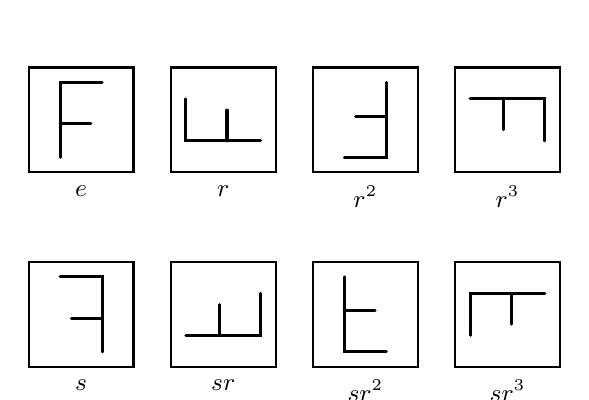
\begin{tikzpicture}[scale=0.95]
  \def\Fsym{\draw[line width=1.1pt, line cap=round]
      (-0.28,-0.5) -- (-0.28,0.5) -- (0.28,0.5)
      (-0.28,-0.05) -- (0.13,-0.05);}
  \foreach \ang/\lab [count=\i from 0] in {0/e, 90/r, 180/r^2, 270/r^3} {
    \begin{scope}[xshift=\i*1.9cm]
      \draw[thick] (0.05,0.05) rectangle (1.45,1.45);
      \begin{scope}[shift={(0.75,0.75)}]
        \begin{scope}[rotate=\ang]
          \Fsym
        \end{scope}
      \end{scope}
      \node[below, font=\small] at (0.75,0.0) {$\lab$};
    \end{scope}
  }
  \foreach \ang/\lab [count=\i from 0] in {0/s, 90/sr, 180/sr^2, 270/sr^3} {
    \begin{scope}[xshift=\i*1.9cm, yshift=-2.6cm]
      \draw[thick] (0.05,0.05) rectangle (1.45,1.45);
      \begin{scope}[shift={(0.75,0.75)}]
        \begin{scope}[xscale=-1]
          \begin{scope}[rotate=\ang]
            \Fsym
          \end{scope}
        \end{scope}
      \end{scope}
      \node[below, font=\small] at (0.75,0.0) {$\lab$};
    \end{scope}
  }
\end{tikzpicture}
\\[4pt]
{\small 图：正方形（$D_8$）的八个对称。上行为旋转 $e,r,r^2,r^3$；下行为反射 $s,sr,sr^2,sr^3$（分别关于四条对称轴，其中 $s$ 关于竖直轴）；$r$ 是逆时针转 $90^\circ$。}
\end{minipage}
\end{center}


用生成元和关系写成

\[D_{2n}=\langle r,s\mid r^n=s^2=e,\ rs=sr^{-1}\rangle.\]


\begin{center}
\begin{minipage}{0.95\textwidth}
\centering
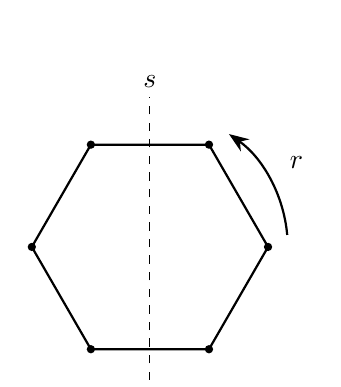
\begin{tikzpicture}[scale=1.0]
  \draw[thick] (0:1.5) \foreach \a in {60,120,180,240,300} { -- (\a:1.5) } -- cycle;
  \foreach \a in {0,60,120,180,240,300} { \fill (\a:1.5) circle (1.5pt); }
  \draw[-{Stealth[length=2.5mm]}, thick] (5:1.75) arc (5:55:1.75);
  \node at (30:2.15) {$r$};
  \draw[dashed] (0,-1.9) -- (0,1.9);
  \node[above] at (0,1.9) {$s$};
\end{tikzpicture}
\\[4pt]
{\small 图：$D_{2n}$ 的生成元——旋转 $r$ 与关于竖直虚线轴的反射 $s$（图中 $n=6$）。}
\end{minipage}
\end{center}


由此可得 $r^ks=sr^{-k}$，于是每个元素都能唯一地写成

\[r^k\quad\text{或}\quad sr^k,\qquad 0\le k<n,\]

即 $D_{2n}=\{e,r,\ldots,r^{n-1},s,sr,\ldots,sr^{n-1}\}$。

例如

\[(sr^2)(sr^5)=s(r^2s)r^5=s(sr^{-2})r^5=r^3.\]

注意 $r^2s=sr^{-2}$，不能把 $r^2s$ 写成 $sr^2$。当 $n\ge3$ 时 $D_{2n}$ 一般不是 Abel 群，例如 $sr=r^{-1}s$。

\subsection{自由群}


给定字母表 $S$。把每个 $s\in S$ 与形式逆记号 $s^{-1}$ 放在一起，$S$ 上的词（word）是有限字符串

\[w=s_1^{\varepsilon_1}s_2^{\varepsilon_2}\cdots s_k^{\varepsilon_k},\qquad s_i\in S,\quad \varepsilon_i\in\{1,-1\},\]

空串（长度为 $0$ 的词，记作 $e$）也允许。

\textbf{相等关系。} 把能通过下面操作互相转化的词视为相等：在词中任意位置插入或删除相邻互逆对，

\[w\,ss^{-1}\,w'\sim w\,w',\qquad w\,s^{-1}s\,w'\sim w\,w'.\]

自由群（free group）$F(S)$ 的元素就是这些词模掉上述等价关系得到的等价类。

\textbf{群运算。} 两个类 $[u]$、$[v]$ 的乘积定义为：各取一个代表词 $u,v$，拼接起来，取拼接词所在的类，

\[[u]\cdot[v]=[uv].\]

换一组代表词不会改变结果：把 $u$ 换成同类词 $u'$，只需对拼接词 $uv$ 的前半段做同样的插入/删除，就得到 $u'v$，所以 $uv$ 与 $u'v$ 同类；对 $v$ 同理。因此乘法是良定义的。

例如 $[ab]\cdot[b^{-1}c]$：拼接得 $ab\,b^{-1}c$，删去 $bb^{-1}$ 得 $ac$，所以乘积是 $[ac]$。

空词的类 $e$ 是单位元。词 $w=s_1^{\varepsilon_1}\cdots s_k^{\varepsilon_k}$ 的逆元是反序并逐个取逆：

\[w^{-1}=s_k^{-\varepsilon_k}\cdots s_1^{-\varepsilon_1},\]

因为 $w\,w^{-1}=s_1^{\varepsilon_1}\cdots s_k^{\varepsilon_k}\,s_k^{-\varepsilon_k}\cdots s_1^{-\varepsilon_1}$ 中的互逆对可以逐对删去，最后剩下空词。

\textbf{自由性。} 自由群中除了由群的性质可推出相等的以外都不相等：例如 $aba^{-1}b^{-1}\ne e$，而 $abb^{-1}a^{-1}=e$。

\subsection{关系与表示}


$\langle r,s\mid r^n=s^2=e,\ rs=sr^{-1}\rangle$ 这种写法叫群的表示（presentation）：竖线左边是生成元（generators），右边是关系（relations）。

对照自由群：$F(r,s)$ 的相等最少——只承认由群的性质推出的相等；在它上面再要求 $r^n=e$、$s^2=e$、$rs=sr^{-1}$ 成立，能推出的相等变多，得到的群正是 $D_{2n}$。

有了关系就可以化简词，例如由 $rs=sr^{-1}$ 得 $r^ks=sr^{-k}$，于是每个元素都能整理成 $r^k$ 或 $sr^k$ 的形式。

\input{sections/03-permutations}
\input{sections/04-subgroups-cosets}
\input{sections/05-normal-subgroups}
\input{sections/06-quotient-groups}
\section{群同态：定义、核与像}


参考：[DF] Dummit–Foote《Abstract Algebra》§1.6（定义）、§3.1（Proposition 1）、§3.3（Corollary 17）；[DS]《离散数学与结构》§9.5。

\subsection{定义}


设 $G,H$ 是群。映射 $\varphi:G\to H$ 若对任意 $a,b\in G$ 满足

\[\varphi(ab)=\varphi(a)\varphi(b),\]

称为群同态（homomorphism）。若 $\varphi$ 是单射，称为单同态；若为满射，称为满同态；若既单又满（即双射），称为同构（isomorphism），记 $G\cong H$。

\subsection{同态保持的结构}


设 $e_G,e_H$ 分别是两群的单位元。由

\[\varphi(e_G)=\varphi(e_Ge_G)=\varphi(e_G)^2\]

和消去律得 $\varphi(e_G)=e_H$。又

\[e_H=\varphi(e_G)=\varphi(aa^{-1})=\varphi(a)\varphi(a^{-1}),\]

所以 $\varphi(a^{-1})=\varphi(a)^{-1}$。归纳得 $\varphi(a^n)=\varphi(a)^n$（$n\in\mathbb Z$）。因此若 $|a|$ 有限，则 $|\varphi(a)|$ 整除 $|a|$；同构保持元素的阶。

\subsection{核与像}


\[ \operatorname{im}\varphi=\varphi(G)=\{\varphi(g):g\in G\}\le H,\qquad \ker\varphi=\{g\in G:\varphi(g)=e_H\}\le G. \]

像（image）是目标群中被映到的部分，核（kernel）是被映到单位元的元素。

验证 $\ker\varphi\le G$：对 $g,g'\in\ker\varphi$，

\[\varphi\bigl(g\,(g')^{-1}\bigr)=\varphi(g)\,\varphi(g')^{-1}=e_He_H^{-1}=e_H,\]

由子群判定准则即得。

核是正规子群：若 $k\in\ker\varphi$，$g\in G$，则

\[\varphi(gkg^{-1})=\varphi(g)\,e_H\,\varphi(g)^{-1}=e_H,\]

所以 $gkg^{-1}\in\ker\varphi$，即 $\ker\varphi\trianglelefteq G$。

\subsection{单射与满射}


同态满足

\[\varphi\ \text{单射}\iff\ker\varphi=\{e_G\}.\]

证明：若 $\varphi(a)=\varphi(b)$，则

\[\varphi(ab^{-1})=\varphi(a)\varphi(b)^{-1}=e_H,\]

即 $ab^{-1}\in\ker\varphi$；核平凡时 $a=b$。反之若 $k\in\ker\varphi$，则 $\varphi(k)=\varphi(e_G)$，单射给出 $k=e_G$。满射等价于 $\operatorname{im}\varphi=H$。

\subsection{例}


1. 行列式 $\det:GL_n(F)\to F^\times$ 是满同态，核为
\[\operatorname{SL}_n(F)=\{A\in GL_n(F):\det A=1\}.\]
对任意 $c\in F^\times$，矩阵 $\operatorname{diag}(c,1,\ldots,1)$ 的行列式是 $c$，所以满射。

2. 对 $N\trianglelefteq G$，映射 $\pi:G\to G/N$，$\pi(g)=gN$，是满同态且 $\ker\pi=N$。

\subsection{同态的纤维}


对 $h\in\operatorname{im}\varphi$，纤维（fiber）$\varphi^{-1}(h)$ 是核的一个陪集：

\[\varphi^{-1}(h)=g\ker\varphi\qquad(\text{任取 } g \text{ 使 } \varphi(g)=h).\]

因为 $x\in\varphi^{-1}(h)\iff\varphi(g^{-1}x)=e_H\iff g^{-1}x\in\ker\varphi$。于是同态把定义域按核的陪集分块，这正是第一同构定理的直观。


\begin{center}
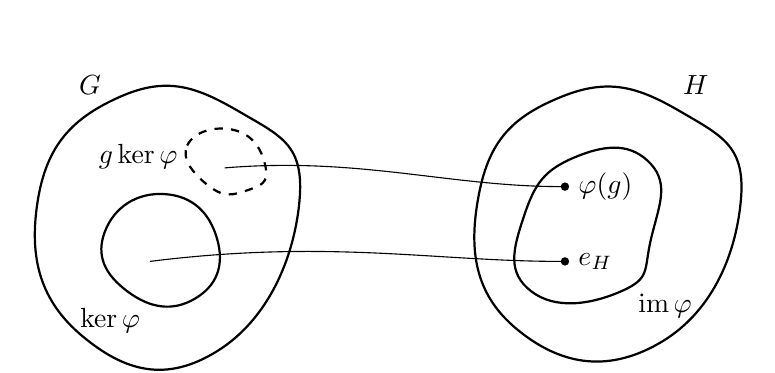
\begin{tikzpicture}[scale=0.95]
  \draw[thick] plot[smooth cycle, tension=0.85] coordinates {(-2.9,-1.5) (-3.5,0.3) (-2.4,1.7) (-0.8,1.5) (0.0,0.3) (-1.1,-1.7)};
  \draw[thick] plot[smooth cycle, tension=0.85] coordinates {(2.9,-1.4) (2.4,0.4) (3.5,1.7) (5.1,1.5) (5.9,0.3) (4.8,-1.6)};
  \node[above] at (-2.8,1.6) {$G$};
  \node[above] at (5.3,1.6) {$H$};
  \draw[thick] plot[smooth cycle, tension=0.9] coordinates {(-2.3,-0.9) (-2.6,-0.1) (-1.8,0.4) (-1.1,-0.2) (-1.4,-1.0)};
  \node[below left] at (-2.0,-1.0) {$\ker\varphi$};
  \draw[thick,dashed] plot[smooth cycle, tension=0.9] coordinates {(-1.2,0.5) (-1.5,1.05) (-0.85,1.25) (-0.45,0.75) (-0.7,0.45)};
  \node[left] at (-1.5,0.9) {$g\ker\varphi$};
  \draw (-2.0,-0.5) .. controls (0.4,-0.2) and (1.8,-0.5) .. (3.5,-0.5);
  \fill (3.55,-0.5) circle (1.6pt);
  \node[right] at (3.6,-0.5) {$e_H$};
  \draw (-1.0,0.75) .. controls (0.8,0.9) and (2.0,0.5) .. (3.5,0.5);
  \fill (3.55,0.5) circle (1.6pt);
  \node[right] at (3.6,0.5) {$\varphi(g)$};
  \draw[thick] plot[smooth cycle, tension=0.9] coordinates {(3.1,-0.9) (3.0,0.1) (3.7,0.9) (4.7,0.8) (4.7,-0.2) (4.3,-0.9)};
  \node[below right] at (4.4,-0.8) {$\operatorname{im}\varphi$};
\end{tikzpicture}
\\[4pt]
{\small 图：同态把每个陪集（纤维）压成一点：$\ker\varphi$ 压到 $e_H$，陪集 $g\ker\varphi$ 压到 $\varphi(g)$。}
\end{center}

\section{第一同构定理（First Isomorphism Theorem）}


参考：[DF] Dummit–Foote《Abstract Algebra》§3.3（Theorem 16、Corollary 17）；[DS]《离散数学与结构》§9.5。

\subsection{定理}


设 $\varphi:G\to H$ 是群同态，则 $\ker\varphi\trianglelefteq G$，且

\[G/\ker\varphi\cong\operatorname{im}\varphi.\]

若 $\varphi$ 是满射，右边就是 $H$，常写成 $G/\ker\varphi\cong H$。

这条定理就是说：$\varphi$ 把核里的元素全压到单位元；把每个陪集都缩成一点，$G$ 剩下的结构和 $\operatorname{im}\varphi$ 完全一样。例如 $\varphi:\mathbb Z_4\to\mathbb Z_2$，$k\mapsto k\bmod 2$：核是 $\{0,2\}$，把 $\{0,2\}$ 与 $\{1,3\}$ 各自压成一个点，$\mathbb Z_4$ 就只剩两个点，正好是 $\mathbb Z_2$。

\subsection{证明}


令 $N=\ker\varphi$，定义

\[\overline\varphi:G/N\longrightarrow\operatorname{im}\varphi,\qquad \overline\varphi(gN)=\varphi(g).\]

需要验证四点。

\textbf{良定义。} 若 $gN=g'N$，则 $g^{-1}g'\in N$，所以 $\varphi(g^{-1}g')=e_H$，即 $\varphi(g)^{-1}\varphi(g')=e_H$，从而 $\varphi(g)=\varphi(g')$。同一个陪集的代表元给出同一个像。

\textbf{同态。} 对 $gN,g'N\in G/N$，

\[\overline\varphi((gN)(g'N))=\overline\varphi(gg'N)=\varphi(gg')=\varphi(g)\varphi(g')=\overline\varphi(gN)\overline\varphi(g'N).\]

\textbf{满射。} 任取 $y\in\operatorname{im}\varphi$，有 $y=\varphi(g)=\overline\varphi(gN)$。

\textbf{单射。} 若 $\overline\varphi(gN)=e_H$，则 $\varphi(g)=e_H$，即 $g\in N$，所以 $gN=N$ 是单位元，核平凡。

于是 $\overline\varphi$ 是同构，定理得证。

\subsection{例}


行列式 $\det:GL_n(F)\to F^\times$ 是满同态，核为 $SL_n(F)$。代入第一同构定理得

\[GL_n(F)/SL_n(F)\cong F^\times.\]

\subsection{推论}


\begin{itemize}
\item $\varphi$ 单射 $\iff\ker\varphi=\{e\}$；此时 $\varphi$ 给出 $G\cong\operatorname{im}\varphi$。
\item $\varphi$ 满射时 $G/\ker\varphi\cong H$。
\item 若 $G$ 有限，则 $|G|=|\ker\varphi|\cdot|\operatorname{im}\varphi|$；一般地 $|G/\ker\varphi|=|\operatorname{im}\varphi|$。
\item 对任意 $g,g'$ 有 $\varphi(g)=\varphi(g')\iff g\ker\varphi=g'\ker\varphi$，即每个纤维都是核的陪集。把每个纤维缩成一点，就得到 $G/\ker\varphi\cong\operatorname{im}\varphi$。
\end{itemize}

\input{sections/09-isomorphism-theorems}

\section*{参考文献}
\begin{itemize}
\item \textbf{[DF]} D. S. Dummit, R. M. Foote. \emph{Abstract Algebra}, 3rd ed. John Wiley \& Sons, 2004.
\item \textbf{[DS]} 邓小铁、王畅. 《离散数学与结构》. 未定稿, 2023.
\end{itemize}
\end{document}
